\chapter{Experimental Results}
\label{capitolo5}
\thispagestyle{empty}

\section{Dataset Acquisition}

The visual dataset has been collected in simulated environments from Matterport3D dataset \cite{matterport} through the modified version of Gibson (described in Sec. \ref{sec:new_gibson_version}). The entire dataset is publicly available\footnote{The dataset is downloadable \href{https://drive.google.com/file/d/1BqjBpobjKTomFjDkzhWjmCryAXOEluO2/view?usp=sharing}{here}.}The positions from which the examples are acquired are extracted from the Pose Selector, described in Sec \ref{sec:pose_estimator}. We select a set $E$ of $10$ worlds of Matterport3D dataset, where $E = \{\text{house1}, \text{house2}, \text{house7}, \text{house9}, \text{house10}, \text{house13}, \text{house15}, \text{house20}, \\ \text{house21},  \text{house22}\}$. The dataset's acquisition procedure, previously described in Sec. \ref{sec:dataset_labeling}, is now formalized by reporting the various steps and specifying the hyper-parameters' values. The collection algorithm works as follows:

\begin{enumerate}
	\item we start a simulation run with Gibson for each environment $e \in E$, where the virtualized agent is a Turtlebot2 \cite{turtlebot2};
	\item for each environment we select a set of positions through the Pose Estimator module, by setting \textsf{interval} $= 1.00m$. This means that the selected positions are spaced $1.00m$ from each other in the Voronoi graph created by Pose Estimator;
	\item during the simulation run, the robot is positioned in each location and we collect a pool of examples changing the robot orientation and the height with respect to the floor. We select a set of height values $H = \{0.10m, 0.70m\}$ and a set of 8 rotation angles $O = \{0^{\circ}, 45^{\circ}, 90^{\circ}, 135^{\circ}, 180^{\circ}, 225^{\circ}, 270^{\circ}, 315^{\circ}\}$;
	\item for each position, we collect an example for every pair height-orientation in the Cartesian product $H \times O = \{(h, o) \mid h \in H, o \in O\}$. Since $|H \times O| = 16$, we collect 16 examples for each location extracted in the previous step;
	\item as mentioned in Sec \ref{sec:dataset_labeling}, an examples is initially composed by the data provided by Gibson: an RGB image, depth data, and a semantic information contained in another RGB image;
	\item a human operator parses all the positive examples whit a dedicated tool in order to fix the bounding boxes found with the semantic annotated images, to specify the label (which means close or open doors) for each bounding box, and to highlight the implicit doors which are not tagged. During this manual labeling procedure, the user also discards the bounding boxes around not valid objects of interest, that are doors too close or too far in the RGB image. In particular, we discarded a door too close to the acquisition position considering the depth data: if the average distance is less that $0.30 m$, the bounding box is not displayed. Likewise, the doors too far with respect to the robot position are not considered if they cover less than $2,5\%$ of the total semantic image. In such situations, the tool we developed does not displays the bounding boxes. If an image has no valid doors, the entire example is discarded. Another important goal of the manual labeling procedure is to remove the corrupted or malformed images produced by Gibson;
	\item with the same tool, a human operator checks also the negative images to discard the examples with wrong RGB images; 
	\item the labeling tool automatically saves the checked examples in a new dataset folder. Finally, each example is composed by an RGB image, the depth data, and an array that contains the bounding boxes coordinates and their labels (that indicate the door's status). 
\end{enumerate}

The dataset is managed using the \textit{generic-dataset} packaged described in Sec. \ref{sec:generic_dataset}. This framework organizes the dataset persistence directory-tree by Fig. \ref{fig:organization_dataset}.

\begin{figure}[h!]
	\centering
	\begin{minipage}{7cm}
		\dirtree{%
			.1 MAIN\_DATASET\_FOLDER.
			.2 house1.
			.3 1.
			.4 rgb\_image.
			.5 rgb\_image\_rc\_ac.png.
			.5 rgb\_image\_rc\_ac.png.
			.5 \vdots.
			.4 depth\_data.
			.5 \vdots.
			.4 bounding\_boxes.
			.5 \vdots.
			.3 0.
			.4 \vdots.
			.3 \vdots.
			.2 house2.
			.3 \vdots.
			.2 \vdots.
		}
	\end{minipage}
	\caption{The structure of the visual dataset collected in this thesis. }
	\label{fig:organization_dataset}
\end{figure} 

Table \ref{tab:dataset_examples_number} reports the number of examples acquired for each environment $e \in E$, that compose the dataset we collected.

\begin{table}[h!]
	\centering
	\begin{tabular}{cccc}

	\toprule
	\textbf{Env. name} & \textbf{Positive examples} & \textbf{Negative examples} & \textbf{Total
		examples}\tabularnewline
	\midrule
	house1 & 350 & 363 & 713\tabularnewline
	house2 & 482 & 529 & 1011\tabularnewline
	house7 & 358 & 227 & 585\tabularnewline
	house9 & 774 & 410 & 1184\tabularnewline
	house10 & 446 & 308 & 754\tabularnewline
	house13 & 413 & 230 & 643\tabularnewline
	house15 & 652 & 423 & 1075\tabularnewline
	house20 & 408 & 350 & 758\tabularnewline
	house21 & 826 & 551 & 1377\tabularnewline
	house22 & 748 & 515 & 1263\tabularnewline
	\bottomrule
	\end{tabular}
	\caption{The number of examples for every environment $e \in E$.}
	\label{tab:dataset_examples_number}
\end{table}

\section{DETR Configuration}

As mentioned in Sec. \ref{sec:doors_detector}, the doors detector module proposed in this thesis is built using DETR \cite{detr}. As a reminder, DETR's architecture (described in Sec. \ref{sec:sec:detrarchitecture}) is composed by a CNN backbone (ResNet \cite{resnet}) which  provides a low dimensional representation of it. Then, the features extracted are fed into a Transformer \cite{transformer} to capture the relationships between them by reasoning over the entire image as context. Finally, the bounding boxes coordinates are inferred by a 4-layer perceptron while their labels are extracted through a linear classifier. In the following paragraphs, we describe in detail the configuration of DETR we use to run our experiments. We starts discussing the architecture of DETR. Then, we proceed describing the parameters' initialization and, finally, we report the hyper-parameter used for the training of DETR

\paragraph{DETR Architecture}
\citeauthor{detr} \cite{detr} propose 4 versions of DETR. The first one is composed by a ResNet-50 while the second has a ResNet-101 as feature extractors. The authors called these models DETR and DETR-R101 respectively. Then, the authors propose other two architectures starting from both DETR and DETR-R101. Following the work proposed in \cite{fullyconvolutional}, the authors of DETR increase the feature resolution by
adding a dilation to the last stage of the backbone and removing a stride from
the first convolution of this stage. The corresponding models are called respectively DETR-DC5 and DETR-DC5-R101. This modification
increases the resolution by a factor of two, thus improving performance for small
objects, at the cost of a 16x higher cost in the self-attentions of the encoder,
leading to an overall 2x increase in computational cost. This modification
increases the resolution by a factor of two, thus improving performance for small
objects, at the cost of a 16x factor in the self-attentions of the encoder,
leading to an overall 2x increase in computational cost. A full comparison of
FLOPs (number of floating point operations per second), FPS (frame per second), and parameters' number of these models is given in Table \ref{tab:detr_models_flops}. The authors calculate the FLOPS for first 100 images in the COCO 2017 validation set using tool \textsf{flop\_count\_operators} from Detectron2 \cite{detectron2}. We use the standard version of DETR to build the doors detector: the model's efficiency is crucial in a robotic context and the modified versions of DETR increase a lot the inference time and the memory consumed. 

\begin{table}[h!]
	\centering
	\begin{tabular}{cccc}
		
		\toprule
		\textbf{Model name} & \textbf{GFLOPS} & \textbf{FPS} & \textbf{Paramaters} \tabularnewline
		\midrule
		DETR & 86 & 28 & 41M\tabularnewline
		DETR-DC5 & 187 & 12 & 41M\tabularnewline
		DETR-R101 & 152 & 20 & 60M\tabularnewline
		DETR-DC5-R101 & 233 & 10 & 60M\tabularnewline
		\bottomrule
	\end{tabular}
	\caption{The comparison between the four architecture of DETR. Table from \cite{detr}.}
	\label{tab:detr_models_flops}
\end{table}

\paragraph{DETR Initialization}
We do not retrain the entire model but we load the pre-trained version of DETR furnished by the authors. This is because training DETR from scratch is unfeasible. First of all, as reported in \cite{surveytransformer}, the Transformers used in Computer Vision need wide training datasets. As a prove, DETR is trained for 300 epochs using the COCO 2017 dataset \cite{coco} which contains for about 118K of training images. This procedure takes 3 days on a cluster with 16 Tesla V100 GPUs and a batch size of 64 (4 images for each GPU). Since we have a small doors dataset (with for about 8K examples) and a limited computing power, we fine-tune DETR with a few data to resolve a more refined task (detecting doors). Fine-tuning a model pre-trained with a dataset like Imagenet \cite{imagenet} has become a common technique for solving computer vision tasks \cite{verydeepimagenet, resnet, fasterrcnn, yolo, yolov2}. We adopt the same strategy, with the difference that DETR is pre-trained using COCO dataset.

\paragraph{DETR Hyper-Parameters}
Now, we describe in detail the setting of the hyper-parameters used for training the model. We train DETR using the AdamW  \cite{adamw} optimizer implemented in PyTorch. We set AdamW with a \textsf{weight\_decay} of $1^{-4}$. The backbone and the transformers are treated slightly differently.  We train the CNN backbone with a learning rate of $10^{-6}$, while the learning rate of the Transformer is set at $10^{-5}$. The authors observe that having the backbone learning rate roughly an order of magnitude smaller than the rest of the network is important to stabilize training, especially in the first few epochs. 

As reported in Sec. \ref{sec:detrlosses}, the loss function for bounding box regression is a linear combination of $\ell_1$ and generalized IoU \cite{generalizediou} losses (Eq. \ref{eq:bounding_box_loss}). We set $\lambda_{iou} = 2$ and $\lambda_{L1} = 5$.

Another important hyper-parameter is the number of object queries. As specified in Sec. \ref{sec:detrarchitecture}, the module produce a detection for each object queries. In the original article of DETR \cite{detr}, the total number of object queries is  $N = 100$. This because, as specified by the authors, $N$ must be greater than the maximum number of objects instances in an image (the images of COCO contain up to 70 distinct objects). In our dataset, the maximum number of doors in an image is 3, so we set $N = 10$.

\paragraph{Data Augmentation} DETR \cite{detr} is a wide model that requires a huge amount of training data to converge. To overcome this issue, the authors perform an intense data augmentation of the COCO's images used for DETR's training. Another purpose of the data augmentation technique is to generalize well the problem by producing new images starting from the original ones. In this way, the model learns from different images increasing in accuracy and preventing overfitting. 

The data augmentation applied to each training image is composed by the following operations:

\begin{enumerate}
	\item \textbf{horizontal flip:} at first, the authors apply a horizontal flip to the image with a probability of $0.5$;
	\item \textbf{random select:} now, the data augmentation proceeds choosing one of the following algorithms with a probability of $0.5$:
	\begin{enumerate}
		\item \textbf{random resize:} the image is randomly resized such that the shortest side is at least 480 and at most 800 pixels while the longest at most 1333;
		\item \textbf{random size crop:} the image, which is initially resized with the same procedure of the previous operation, is cropped to a random rectangular patch (with random sizes) which is then resized again;
	\end{enumerate} 
	\item finally, the image is normalized. Normalizing the images means transforming the images into such values that the mean and standard deviation of the image become 0.0 and 1.0 respectively. First of all, an image $W \times H \times 3$ is converted to a tensor with shape $3 \times H \times W $ and the integer pixels are scaled in the $[0.0, 1.0]$ interval. Then, each input channel is subtracted by the channel mean and then the result is divided by the channel standard deviation. The channels' mean and standard deviation used by the authors are calculated over the Imagenet dataset \cite{imagenet}.
\end{enumerate}

During the firsts experiments, we argue that this massively data augmentation is not appropriate in the context of this thesis. First of all, we use the pre-trained DETR version on COCO 2017 dataset, so the model already has a good initialization of the weights. Furthermore, we use a dataset less than one order of magnitude with respect to COCO. This means that we do not have enough examples for making a data modification like those performed in the original train of DETR. Another important issue regards the crop procedure with respect to the our objects of interest. In the context of this thesis, we aim to detect open or closed doors, that are typically big objects in images. By random cropping a frame, the door's features may be insufficient for a successful model's training. For these reasons, we perform a reduced data augmentation. With a probability of $0.5$, we modify the image with a random horizontal flip followed by a random resize operation; otherwise, the image is not modified. Finally, we normalize the frame with mean and standard deviation of Imagenet dataset. Since our images are smaller ($256 \times 256 \times 3$) than those of COCO, the random resize is performed in a different range, between 256 and 576 pixels. 

\section{DETR Analysis}

Before proceeding with the evaluation of DETR over the collected dataset, we test the proposed doors detector with a well known doors dataset, called \textit{DeepDoors2} \cite{deepdoors2}, which is freely available on Github\footnote{The DeepDoors2 Github page: \url{https://github.com/gasparramoa/DeepDoors2}.}. We perform this experiment to understand if DETR is trainable with a smaller dataset than COCO and to verify if it obtains good results in a doors detection task. In the following sub-sections, we describe in detail the DeepDoors2 dataset proposed in \cite{deepdoors2} and how we modify it to better approach the requirements of the task addressed by this thesis. Then, we report the results obtained by the doors detector we proposed if trained with the improved version of DeepDoors2. Finally, we further analyze the DETR's performance by visualizing the detections produced by the trained model using t-SNE \cite{tsne}.

\section{DeepDoors2 Dataset}
DeepDoors2 is a visual dataset which contains 3000 labeled examples composed by  RGB images (with dimension of $480 \times 640 \times 3$), depth data, and the relative semantic information encoded in another RGB images. The labels provided by the authors indicates also the doors' status, which can be open, semi-open, and closed (Fig. \ref{fig: open_semi_closed}). The examples are equally divided over these doors' categories.  This dataset is constituted by 3 parts, a 2D and 3D image classification part, a semantic segmentation part and an object detection part. For the first two parts, the authors use their previous
dataset, published in \cite{deepdoors1}, and improve it by collecting more data and annotating more images. The third part was built by labeling the image of the classification part. This dataset was captured in different indoor environments (universities, public spaces, and houses) using a portable system constituted by a Raspberry Pi 3 B+ with a 3D Realsense Camera, model D435. The authors captured several images of doors and their surroundings with different textures and sizes, sometimes obstructed by obstacles (e.g. chairs, tables, furniture, and even persons). The authors also changed the pose to get different perspectives on the same door. 

\begin{figure}[h!]
	\begin{subfigure}[b]{0.32\linewidth}
		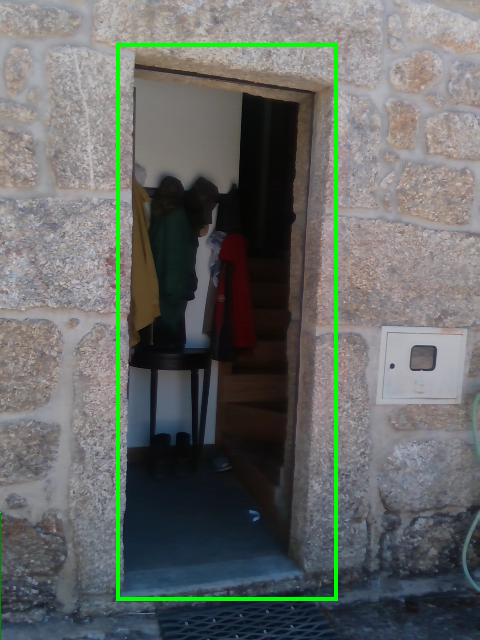
\includegraphics[width=\linewidth]{images/deep_doors_2_open.png}
		\caption{}
	\end{subfigure}
	\hfil
	\begin{subfigure}[b]{0.32\linewidth}
		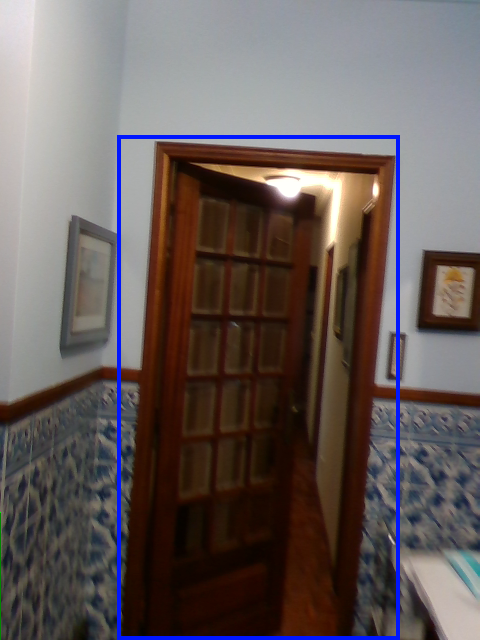
\includegraphics[width=\linewidth]{images/deep_doors_2_semiopen.png}
		\caption{}
	\end{subfigure}
	\hfil
	\begin{subfigure}[b]{0.32\linewidth}
		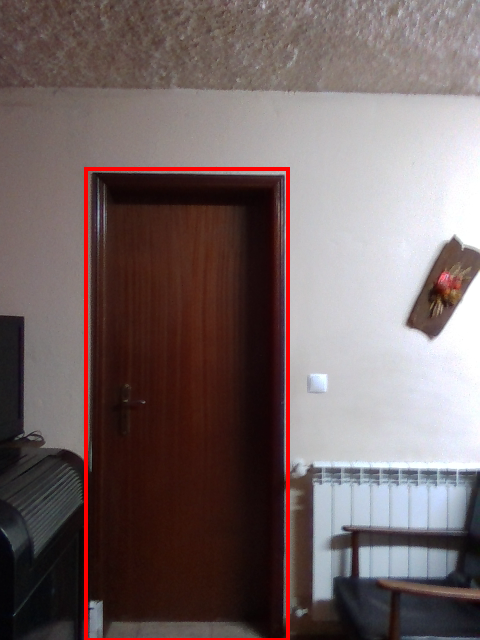
\includegraphics[width=\linewidth]{images/deep_doors_2_closed.png}
		\caption{}
	\end{subfigure}
	\caption{Labeled images from DeepDoors2 dataset. (a) An open door, (b) a semi-open door, and (c) a closed door. Green, blue, and red bounding boxes represent open, semi-open, and closed doors respectively.}
	\label{fig: open_semi_closed}
\end{figure}

The object detection part of DeepDoors2 dataset is annotated with an automatic procedure that finds bounding boxes around doors using the semantic data. The labeling algorithm implemented by the authors finds a single door for each image, but we argue that a single example can depict multiple doors instances with different statues (Fig. \ref{fig:relabeling_deepdoors2}). Due to this fact, we manually re-label the entire dataset with the visual tool described in Sec. \ref{sec:dataset_labeling}. Furthermore, we re-organize the dataset according to the standard defined by the \textit{generic-dataset} framework reported in Sec. \ref{sec:generic_dataset}. We release the re-labeled version of DeepDoors2 dataset\footnote{The DeepDoors2 re-labeled dataset can be downloaded \href{https://drive.google.com/file/d/1wSmFUHF9aSJkomwFdOmepMevBvkRpf3D/view?usp=sharing}{here}.} and the necessary Python code\footnote{The DeepDoors2 re-labeled source code: \url{https://github.com/micheleantonazzi/deep-doors-2-labelled}.} to manage it. The final DeepDoors2 dataset is composed oh 2998 examples, while each of them include an RGB image with dimension $480 \times 640 \times 3$, a matrix $480 \times 640$ which contains the depth data, and a list with the bounding boxes' coordinates and the relative labels (open, semi-open, or closed door). 

\begin{figure}[h!]
	\centering
	\begin{subfigure}[b]{\linewidth}
		\hfil
		\begin{subfigure}[b]{0.26\linewidth}
			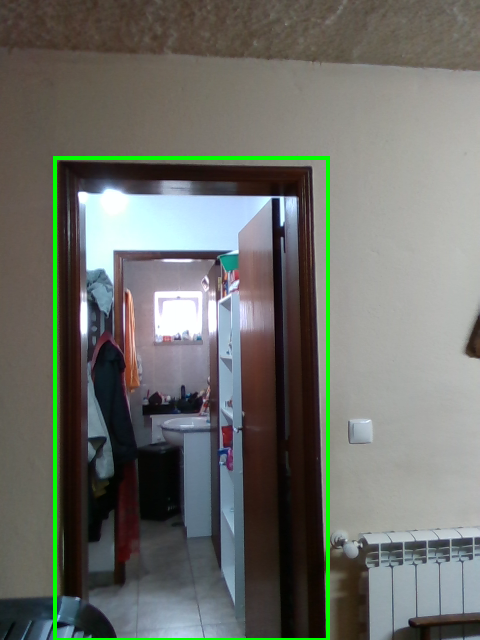
\includegraphics[width=\linewidth]{images/deep_doors_2_labeling1.png}
		\end{subfigure}
		\hfil
		\begin{subfigure}[b]{0.26\linewidth}
			
\includegraphics[width=\linewidth]{images/deep_doors_2_labeling1_semantic.png}
		\end{subfigure}
		\hfil
		\begin{subfigure}[b]{0.26\linewidth}
			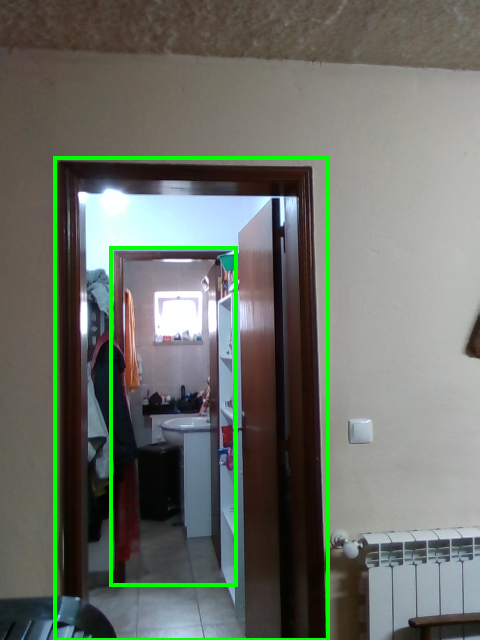
\includegraphics[width=\linewidth]{images/deep_doors_2_labeling1_correct.png}
		\end{subfigure}
		\hfil
		\caption{}
	\end{subfigure}
	\newline
	\begin{subfigure}[b]{\linewidth}
		\hfil
		\begin{subfigure}[b]{0.26\linewidth}
			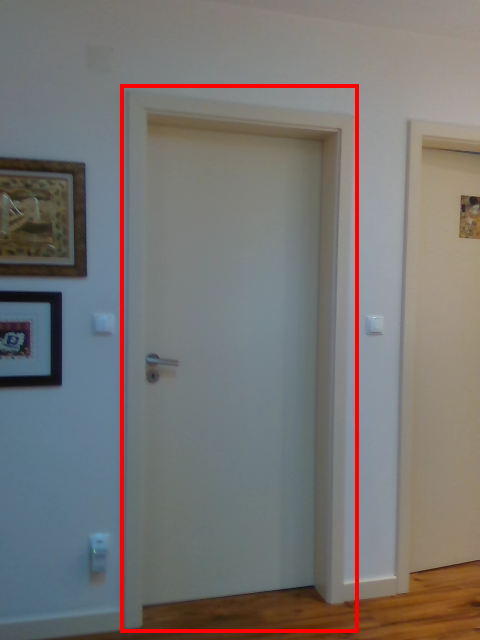
\includegraphics[width=\linewidth]{images/deep_doors_2_labeling2.png}
		\end{subfigure}
		\hfil
		\begin{subfigure}[b]{0.26\linewidth}
			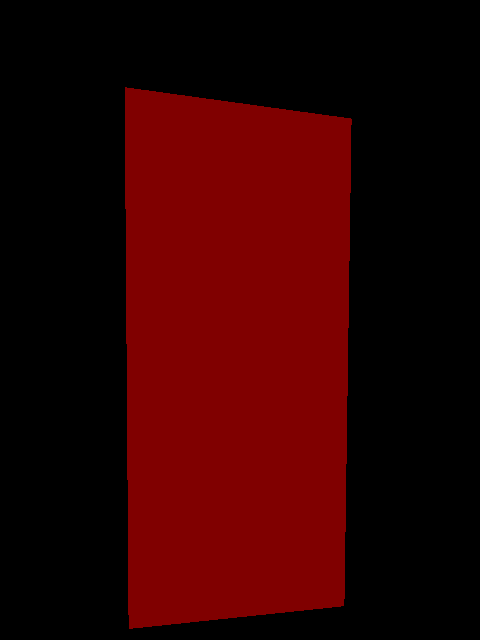
\includegraphics[width=\linewidth]{images/deep_doors_2_labeling2_semantic.png}
		\end{subfigure}
		\hfil
		\begin{subfigure}[b]{0.26\linewidth}
			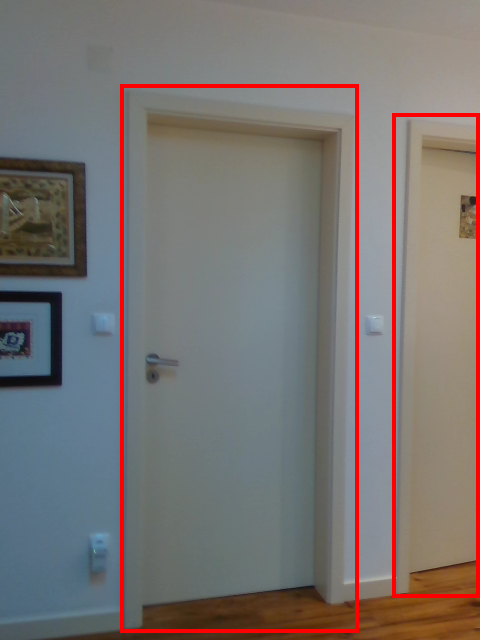
\includegraphics[width=\linewidth]{images/deep_doors_2_labeling2_correct.png}
		\end{subfigure}
	\hfil
		\caption{}
	\end{subfigure}
	\caption{Two examples of wrong labeled images from the original version of DeepDoors2 dataset. The left figures in each row represents the bounding boxes found with the depth data encoded in the middle images. The figures on the right depict the fixed labeled images of our version DeepDoors2.}
	\label{fig:relabeling_deepdoors2}
\end{figure}

\subsection{DETR's Performance on DeepDoors2}

Before proceeding with other experiments, we test DETR on the relabeled version of DeepDoors2 to verify if it converges with such a small dataset and if it has acceptable performance in a doors detection task. We randomly split the dataset into a training set of the $80\%$ of examples and a test set with the remaining ones. We train DETR for 40 epochs with a batch size of 1. We report the DETR loss function (Eq. \ref{eq:detr_loss}) during training both for train and test sets in Fig. \ref{fig:deep_doors2_loss}.

\begin{figure}[h!]
	\centering
	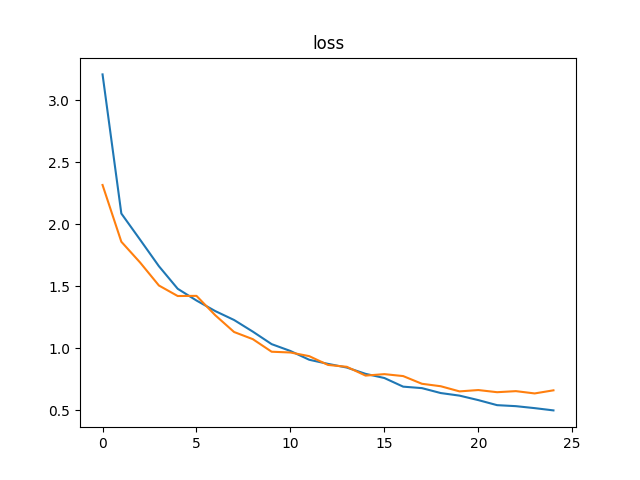
\includegraphics[width=\linewidth]{images/deep_doors_2_loss.png}
	\caption{The loss function during the training of DETR.}
	\label{fig:deep_doors2_loss}
\end{figure}

We evaluate the trained version of DETR with the Pascal VOC metric \cite{pascal} as described in Sec. \ref{sec:model_evaluator}. We set the \textsf{iou\_threshold}$ = 0.9$ and the \textsf{confidence\_threshold} $= 0.5$. Table \ref{tab:deep_doors2_results} reports the AP score for each object category (open, semi-open, and closed doors) and the data to calculate it, such as the total number of the ground-truth bounding boxes, the true positive, and the false positive detections performed by the model. The plot of the interpolated precision/recall curves for each category is shown in Fig. \ref{fig:deep_doors2_ap_plot}.

\begin{table}[h!]
	\centering
	\begin{tabular}{cccccc}
		
		\toprule
		\textbf{Label} & \textbf{AP} & \textbf{N. Positives} & \textbf{TP} & \textbf{FP} & \textbf{FN}\tabularnewline
		\midrule
		Closed door (0) & 0.90 & 234 & 214 & 45 & 20 \tabularnewline
		Semi-open door (1) & 0.83 & 198 & 169 & 33 & 29 \tabularnewline
		Open door (2) & 0.85 & 243 & 214 & 66 & 29 \tabularnewline
		\bottomrule
	\end{tabular}
	\caption{The performance of DETR trained on the DeepDoors2 dataset.}
	\label{tab:deep_doors2_results}
\end{table}

\begin{figure}[h!]
	\centering
	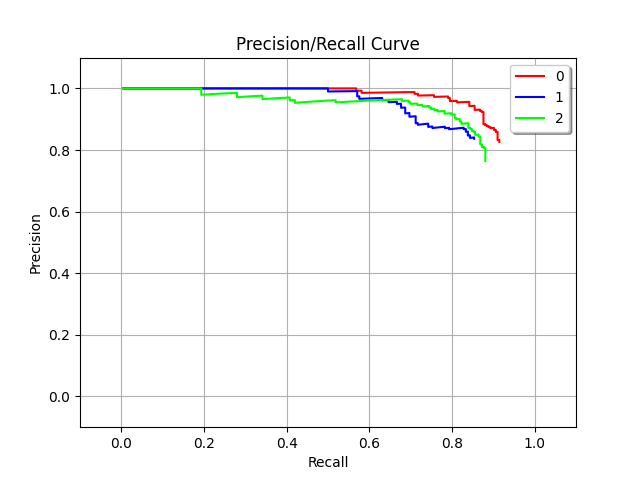
\includegraphics[width=\linewidth]{images/deep_doors_2_precision_recall.png}
	\caption{The interpolated precision/recall curves about open, semi-open, and closes doors, colored in green, blue, and red respectively.}
	\label{fig:deep_doors2_ap_plot}
\end{figure} 

As shown by Fig. \ref{fig:deep_doors2_loss}, the model converges correctly and does not overfit or underfit. Both the training and test error (reported in blue and orange respectively) are low and closed to each other. As reported in Table \ref{tab:deep_doors2_results}, the proposed doors detector reaches a good accuracy for all the three door categories (open, semi-open, and closed). An AP greater that 80 is considered a good in the Computer Vision community.

\subsection{The DETR's Detection Visualization}
As mentioned in Sec. \ref{sec:detrarchitecture}, each object queries produces a detection composed by the bounding box coordinates and the relative label. To further analyze the DETR's performance, we plot in 2D the object queries classified by the Transformers using t-SNE \cite{tsne}. t-SNE (t-distributed Stochastic Neighbor Embedding) is a unsupervised and randomized technique to visualize high-dimensional data by giving each data point a location in a two or three dimensional map. It models each high-dimensional object by a two or three-dimensional point in such a way that similar objects are modeled by nearby points and dissimilar objects are modeled by distant points with high probability. This algorithm is a variation of Stochastic Neighbor Embedding (SNE) \cite{sne}. SNE starts by converting the high-dimensional Euclidean distance between all pairs of data points into conditional probabilities. More formally,  The similarity of data point $x_j$ to data point $x_i$ is the conditional probability $p_{j \mid i}$, where $x_i$ considers $x_j$ as a neighbor in proportion to a Gaussian centered in $x_i$. For nearby data points, $p_{j \mid i}$
is relatively high, whereas for widely separated data points, $p_{j \mid i}$ will be almost infinitesimal. Note that $p_{i \mid i} = 0$. For the low-dimensional counterpart of  $x_i$ and $x_j$ (denoted as $y_i$ and $y_j$), it possible to compute a similar conditional probability  $q_{j \mid i}$.
If the map points $y_i$ and $y_j$ correctly model the similarity between the high-dimensional datapoints $x_i$ and $x_j$, the conditional probabilities $p_{j \mid i}$ and $q_{j \mid i}$ will be equal. Motivated by this observation, SNE aims to find a low-dimensional data representation that minimizes the sum of the mismatches between $p_{j \mid i}$ and $q_{j \mid i}$ of all pairs of data points. A natural way to measure the distance between two probability distributions is the Kullback-Leibler diverge, which the sum is minimized by SNE using a gradient descent method.

Although SNE constructs reasonably good visualizations, it is limited by a cost function that is difficult to optimize because, if $x_i$ is an outlier data point, the value of the joint probabilities $p_{i j}$ (which defines the pairwise similarities in the between $x_i$ and $x_j$ high-dimensional space) is extremely small for all $j$. To overcome this problem, the authors of t-SNE defines the joint probabilities $p_{i j}$ in the high-dimensional space as the symmetrized conditional probability:

\begin{equation}
 p_{i j} = \frac{p_{j \mid i} + p_{i \mid j}}{2n}.
\end{equation}
This ensure that, if $x_i$ is an outlier data point, $\sum_{j} p_{i j} > \frac{1}{2n}$.

Another issue of SNE is the ``crowding problem''. It is difficult to correctly ``scale'' long and short distances of points in low-dimensions. The area in a low-dimensional space that is available to accommodate moderately distant
data points in high-dimensional map will not be nearly large enough compared with the area available to accommodate nearby data points. Otherwise, if we want to model the small distances accurately in the map, most of the points that are at a moderate distance from a data point $i$ will have to be placed much too far away in the two-dimensional map. To overcome this problem, the authors of t-SNE use the Student t-distribution (with a single degree of freedom) instead of the Gaussian in the conversion between Euclidean distance and probability. The Student distribution ``falls'' quickly and has a ``long tail'', so points will not be squashed into a single point. 

The t-SNE algorithm initially calculates the symmetric probabilities $p_{i j}$ between all the high-dimensional data points of a given dataset. Then, it performs multiple iterations in which calculates the low-dimensional affinities values $q_{i j}$, performs the SGD algorithm to optimize the distance between the pairs of $p_{i j}$ and $q_{i j}$.

As previously anticipated, we plot the output embeddings of the Transformer with t-SNE in a two-dimensional space. We train DETR for 40 epochs with a batch size of 1 using 80\% of the examples of the re-labeled version of DeepDoors2. Then, we classify both the training set and the test set (composed the 20\% of the remaining examples) with the trained model, saving the object queries modified by the Transformer. Finally, we clusterize only the predictions with the highest accuracy of every image using the \textit{scikit-image} implementation of t-SNE, by setting 2 different values for perplexity: 30 and 100. Before clusterizing them through t-SNE, we reduce their dimensionality to 50 using the Principal Components Analysis (PCA) \cite{pca}, which projects a data point onto only the first few principal components preserving as much of the data's variation as possible. 

\begin{figure}[h!]
	\centering
	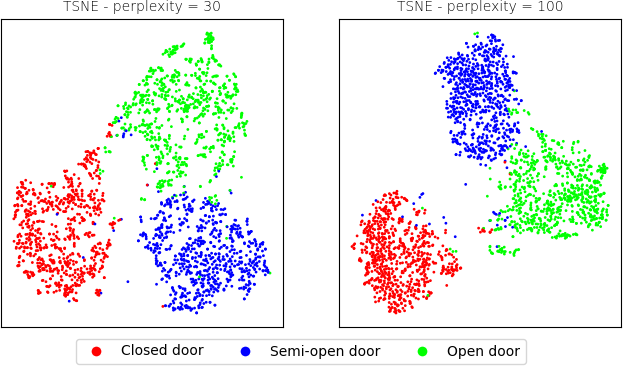
\includegraphics[width=\linewidth]{images/deep_doors_2_tsne_trainset.png}
	\caption{The plot of the Transformer's output embeddings using t-SNE over the training set.}
	\label{fig:tsne_deep_doors2_train}
\end{figure}

\begin{figure}[h!]
	\centering
	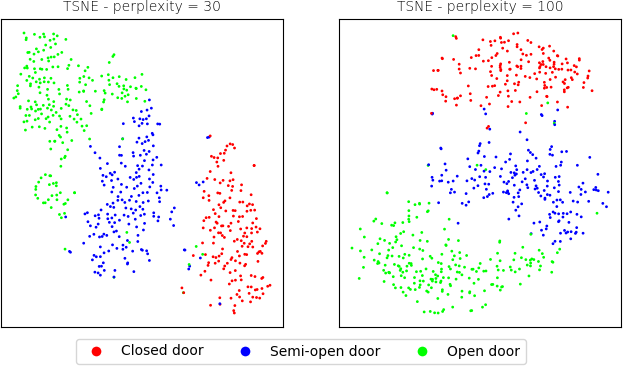
\includegraphics[width=\linewidth]{images/deep_doors_2_tsne_testset.png}
	\caption{The plot of the Transformer's output embeddings using t-SNE over the test set.}
	\label{fig:tsne_deep_doors2_test}
\end{figure}
 
The Figures \ref{fig:tsne_deep_doors2_train} and \ref{fig:tsne_deep_doors2_test} show that DETR produce useful features encoding to separate the open, semi-open, and closed doors. Thanks to t-SNE, we argue that the objects queries classified by the Transformer are clearly separated in three distinct clusters examining both the training and the test sets (as expected looking the good results reported in Tab. \ref{tab:deep_doors2_results}). Since the AP scores are not equals to 1, there are some spurious detections in the t-SNE's plots that likely lead to false positives.
